% --------------------------------------------------------------------------
% Template for IWAENC 2022 papers; to be used with:
%          spconfa4.sty  - ICASSP/ICIP LaTeX style file, and
%          IEEEbib.bst - IEEE bibliography style file.
%
% (Last modified by H. Loellmann, LMS, FAU Erlangen-Nuremberg, Jan. 2020)
%
% --------------------------------------------------------------------------

\documentclass{article}
\usepackage{spconfa4}
\usepackage{amsmath,graphicx}
\usepackage[dvipsnames]{xcolor}
\usepackage{tikz}
\usetikzlibrary{arrows,snakes,backgrounds,matrix,patterns,positioning,fadings}
\usepackage{standalone}
\usepackage{subfig}
\usepackage{upgreek}
\usepackage{nicefrac}
\usepackage{dsfont}
\usepackage{bm}
\usepackage{cancel}
\usepackage{amsbsy}
\usepackage{algorithm}
\usepackage{algpseudocode}
\usepackage{lipsum}
\usepackage{harpoon}
\usepackage{comment}
\newenvironment{note}
 {\par\textcolor{Blue}{\bfseries Note:} \color{Blue}\ignorespaces}
 {\par}
\newenvironment{attention}
 {\par\textcolor{red}{\bfseries Attention:} \color{red}\ignorespaces}
 {\par}
\usepackage{hyperref}
\hypersetup{
	colorlinks,
	linkcolor={blue!80!black},
	citecolor={blue!80!black},
	urlcolor={blue!80!black}
}

\newcommand{\mtxb}[1]{\bm{\mathrm{#1}}}
\newcommand{\T}{{\mathrm{T}}}
\newcommand{\herm}{{\mathrm{H}}}
\newcommand{\ev}[1]{\mathrm{E} \left\lbrace #1 \right\rbrace}
\ninept

% \excludecomment{note}
% \excludecomment{attention}

% IMPORTANT: Add copyright notice by uncommenting the appropriate line
%----------------------------------------------------------
% For papers in which all authors are employed by the US government,
% \copyrightnotice{U.S. Government work not protected by U.S. copyright}

% For papers in which all authors are employed by a Crown government (UK, Canada, and Australia)
% \copyrightnotice{978-1-6654-6867-1/22/\$31.00~\copyright2022 Crown}

% For papers in which all authors are employed by the European Union,
% \copyrightnotice{978-1-6654-6867-1/22/\$31.00~\copyright2022 European Union}

% For all other papers the copyright notice is
\copyrightnotice{978-1-6654-6867-1/22/\$31.00~\copyright2022 IEEE}

% Title.
% ------
\title{DISTRIBUTED CROSS-RELATION-BASED FREQUENCY-DOMAIN\\ BLIND SYSTEM IDENTIFICATION USING ONLINE-ADMM}
%
% Single address.
% ---------------
% \name{M. Blochberger\thanks{This research work was carried out at the ESAT Laboratory of KU Leuven, in the frame of the SOUNDS European Training Network. This project has received funding from the European Union's Horizon 2020 research and innovation programme under the Marie Skłodowska-Curie grant agreement No.\,956369. This research received funding in part from the Research Foundation - Flanders (FWO) grant 12ZD622N as well as from the European Union's Horizon 2020 research and innovation program / ERC Consolidator Grant: SONORA (No.\,773268). This paper reflects only the authors' views and the Union is not liable for any use that may be made of the contained information. Source code available at \url{https://github.com/SOUNDS-RESEARCH/iwaenc2022-admm-bsi}.}, F. Elvander, R. Ali, M. Moonen, J. Østergaard, J. Jensen, T. van Waterschoot}
% \address{KU Leuven\\Department of Electrical Engineering (ESAT)\\STADIUS Center for Dynamical Systems, Signal Processing and Data Analytics \\3001 Leuven, Belgium}

\twoauthors{M. Blochberger, F. Elvander, R. Ali, M. Moonen, T. van Waterschoot
    \thanks{This research work was carried out at the ESAT Laboratory of KU Leuven, in the frame of the SOUNDS European Training Network. This project has received funding from the European Union's Horizon 2020 research and innovation programme under the Marie Skłodowska-Curie grant agreement No.\,956369. This research received funding in part from the Research Foundation - Flanders (FWO) grant 12ZD622N as well as from the European Union's Horizon 2020 research and innovation program / ERC Consolidator Grant: SONORA (No.\,773268). This paper reflects only the authors' views and the Union is not liable for any use that may be made of the contained information. Source code available at \url{https://github.com/SOUNDS-RESEARCH/iwaenc2022-dist-bsi-admm}.}}
        {KU Leuven\\
        Dept. of Electrical Engineering (ESAT)\\
        % STADIUS\\
        3001 Leuven, Belgium}
        {J. Østergaard, J. Jensen}
        {Aalborg University\\
        Dept. of Electronic Systems\\
        % Section on Artificial Intelligence and Sound\\
        9220 Aalborg, Denmark}
%
\begin{document}
%\ninept
%
\maketitle
%
\begin{abstract}
    In this paper, we propose a distributed cross-relation-based adaptive algorithm for blind identification of single-input multiple-output (SIMO) systems in the frequency domain, using the alternating direction method of multipliers (ADMM) in a wireless sensor network (WSN).
    The network consists of a fixed number of nodes each equipped with a processing unit and a sensor that represents an output channel of the SIMO system.
    The proposed algorithm exploits the separability of the cross-channel relations by splitting the multichannel identification problem into sub-problems containing a subset of channels, in a way that is determined by the network topology.
    Each node delivers estimates for the subset of channel frequency responses, which are then combined into a consensus estimate per channel using general-form consensus ADMM in an adaptive updating scheme.
    Using numerical simulations, we show that it is possible to achieve convergence speeds and steady-state misalignment values comparable to fully centralized low-cost frequency-domain algorithms.
\end{abstract}
%
\begin{keywords}
    blind system identification, multichannel signal processing, distributed signal processing, admm, online-admm
\end{keywords}
%
\section{Introduction}
\label{sec:intro}

The problem of blind system identification (BSI), which aims to estimate channel responses of an unknown system without knowing the input signal, has been the subject of extensive research over recent decades.
It was introduced in \cite{satoMethodSelfRecoveringEqualization1975} and various algorithms have been proposed since.
Early algorithms used higher-order statistics \cite{godardSelfRecoveringEqualizationCarrier1980,tongNewApproachBlind1991,mendelTutorialHigherorderStatistics1991} for channel estimation, however, a high computational complexity has motivated research into algorithms that only use second-order statistics.
Such algorithms include the cross-relation (CR) algorithm \cite{langtongBlindIdentificationEqualization1994, guanghanxuLeastsquaresApproachBlind1995}, subspace algorithms \cite{moulinesSubspaceMethodsBlind1995,gannotSubspaceMethodsMultimicrophone2003,diamantarasEfficientSubspaceMethod2008,mayyalaStructureBasedSubspaceMethod2017}, and maximum-likelihood algorithms \cite{yingbohuaFastMaximumLikelihood1996}.
Out of the various multichannel BSI algorithms that have been proposed, adaptive cross-relation-based least-mean-squares (LMS) algorithms in the time and frequency domain are the ones most widely used.
For instance, the normalized multi-channel frequency-domain LMS (NMCFLMS) \cite{huangAdaptiveMultichannelLeast2002,huangClassFrequencydomainAdaptive2003} algorithm is an efficient algorithm utilizing the fast Fourier transform (FFT) which has been extended to include constraints which improve robustness to noise and performance for acoustic impulse responses such as the RNMCFLMS \cite{huNoiseRobustBlind2015}, \(l_p\)-RNMCFLMS \cite{heNoiseRobustFrequencyDomain2018} or phase-constrained-\(l_p\)-RNMCFLMS \cite{joRobustBlindMultichannel2021} algorithms.
On the other hand, the quasi-Netwon algorithm \cite{habetsOnlineQuasiNewtonAlgorithm2010} is a time-domain algorithm that utilizes the Broyden–Fletcher–Goldfarb–Shanno (BFGS) \cite{brodlie1977assessment} method to estimate the Hessian of the problem.

The expanding field of distributed signal processing in wireless sensor networks (WSN) has brought forward algorithms for distributed signal estimation \cite{5483092}, noise control and echo cancellation \cite{9670697}, as well as beamforming \cite{6663655,9670697}. However, research into the task of BSI is limited.
While there exist time-domain algorithms as introduced in \cite{yuDistributedBlindSystem2014,liuDistributedBlindIdentification2016,liuDistributedRecursiveBlind2017}, they do not pose apt comparisons to the frequency-domain algorithm being proposed here.
In this paper, we use the general-form consensus alternating direction method of multipliers (ADMM) \cite{boydDistributedOptimizationStatistical2011} to distribute and solve the optimization problem posed by the task.
We separate the inter-channel cross-relations of the BSI problem according to the network's topology, i.e., each node solves a sub-problem using data from its network neighbors and the entirety of the connected nodes subsequently reach a consensus for the channel frequency responses.
The ADMM update steps are applied in a block processing scheme forming an adaptive algorithm which is also referred to as Online-ADMM \cite{wangOnlineAlternatingDirection2013,hosseiniOnlineDistributedADMM2014}.

As shown in numerical simulations, the resulting algorithm provides good estimation results when compared to state-of-the-art centralized frequency-domain algorithms.

% #############################################################################
% #############################################################################
\section{Problem statement}
\label{sec:problem_statement}

% #############################################################################
\subsection{Signal Model}
\label{ssec:signal_model}
We consider an acoustic SIMO system with input signal \(\mtxb{s}(n) = \begin{bmatrix}
    s(n)&s(n-1)&\ldots&s(n-2L+2)
\end{bmatrix}^{\T}\) and \(M\) output signals \(\x_i(n)= \begin{bmatrix}
    x_i(n)&x_i(n-1)&\ldots&x_i(n-L+1)
\end{bmatrix}^{\T}\)
where \(i \in \Mset \triangleq \{1, \ldots, M\} \).
Each output \(\x_i(n)\) is the convolution of \(\mtxb{s}(n)\) with the respective channel impulse response \(\h_i\) and an additive noise term \(\mtxb{v}_i(n)\), assumed to be zero-mean and uncorrelated with \(\mtxb{s}(n)\).
The signal model is described by
\begin{equation}
    \x_i(n) = \mtxb{H}_i \mtxb{s}(n) + \mtxb{v}_i(n),
\end{equation}
where \(\mtxb{H}_i\) is the \(L \times (2L-1)\) linear convolution matrix of the \(i\)th channel using the elements of \(\h_i\) of length \(L\) which represents the system to be identified.
For the purpose of this paper, the length \(L\) of the impulse responses is assumed to be known.

% #############################################################################
\subsection{Cross-relation Approach}
\label{ssec:cross_rel}
The cross-relation approach for BSI aims to use only the output signals of the system to identify it.
This can be achieved by exploiting the relative channel information when more than one channel is available, and the identifiability conditions \cite{guanghanxuLeastsquaresApproachBlind1995} are satisfied. These conditions are: (i) the channel transfer functions have no common zeros (i.e., the polynomials are not co-prime), and (ii) the covariance matrix of the input signal \(\mtxb{s}(n)\) is of full rank (i.e., the signal has a number of modes \(\geq 2L+1\)).

The fundamental equality of this approach in the noiseless case \(\mtxb{v}_i(n) = 0\) is 
\begin{equation}
    \x_i^{\T}(n) \h_j = \x_j^{\T}(n) \h_i,\quad i,j \in \Mset,\,i\neq j\label{eq:cross_rel:equality_conv}
\end{equation}
which states that the channel output signal convolved with the impulse response of another is equal to the vice-versa as follows from the commutativity property of the convolution.
Left-multiplication with \(\x_i(n)\), assuming deterministic \(\h_j\), and applying the expectation operator to form the covariance matrix \(\R_{ij}(n) = \ev{\x_i(n) \x_j^\T(n)}\), and then combining all cross-relations \eqref{eq:cross_rel:equality_conv} (see e.g., \cite{huangAdaptiveMultichannelLeast2002} for a more detailed derivation) yields the system of equations  
\begin{equation}
    \R \h = \bm{0}, \label{eq:cross_rel:null_space}\\
\end{equation}
where \(\R\) is an \(M L \times M L\) matrix given by
\begin{equation}
    \R = \begin{bmatrix}
        \sum_{i \neq 1} \R_{ii} & -\R_{21} & \cdots & -\R_{M1}\\
        -\R_{12} & \sum_{i \neq 2} \R_{ii} & \cdots & -\R_{M2}\\
        \vdots & \vdots & \ddots & \vdots\\
        -\R_{1M} & -\R_{2M} & \cdots & \sum_{i \neq M} \R_{ii}\\
    \end{bmatrix}\label{eq:cross_rel:data_matrix}
\end{equation}
and \(\h = \begin{bmatrix}
    \h_1^\T & \ldots & \h_M^\T
\end{bmatrix}^\T\).
The derivation is analogous when formulating the problem in the frequency domain.
We denote all frequency-domain variables in bold italic (e.g. \(\Rf\)) compared to the time-domain bold upright (e.g \(\R\)). The derivation involves the frame-based overlap-save technique, working with signal frames \(\x_{i,2L}(m)\) of length \(2L\), frame index \(m\), leading to the system of equations 
\begin{equation}
    \Rf \hf = \bm{0}, \label{eq:frequency_domain:null_space}\\
\end{equation}
where \(\hf = \begin{bmatrix}
    \hf_1^\T & \ldots & \hf_M^\T
\end{bmatrix}^\T \) is a stacked vector of channel frequency responses and the \(M L \times M L\) matrix \(\Rf\) is recursively estimated by \begin{equation}
    \hat{\Rf}(m) = \eta \hat{\Rf}(m-1) + (1-\eta )\tilde{\Rf}(m),
\end{equation}
where \(\eta \in [0,1]\) is an exponential smoothing factor.
The matrix \(\tilde{\Rf}(m)\) is constructed similarly to \eqref{eq:cross_rel:data_matrix}, with \(\sum_{i \neq 1} \tilde{\Rf}_{ii}\) and \(-\tilde{\Rf}_{ij}\) on the diagonal and off-diagonal blocks respectively, where the instantaneous cross-spectrum matrices are defined as
\begin{equation}
    \tilde{\Rf}_{ij}(m) = \bm{X}_{i} (m) \bm{X}_{j}^\herm (m)
\end{equation}
with 
\begin{equation}
    \bm{X}_{i}(m) = \bm{{W}}^{01}_{L \times 2L} \bm{{D}}_{i}(m) \bm{{W}}^{10}_{2L \times L}.
\end{equation}
The matrix \(\bm{{D}}_{i}(m) = \operatorname{diag} \left\{ \operatorname{FFT}_{2L} \left\{ \x_{i,2L}(m) \right\} \right\}\) contains the  signal spectrum on its diagonal and
\begin{align}
    \bm{{W}}_{L \times 2L}^{01} &= \mtxb{F}_{L \times L} \mtxb{W}_{L \times 2L}^{01} \mtxb{F}_{2L \times 2L}^{-1},\\
    \bm{{W}}_{2L \times L}^{10} &= \mtxb{F}_{2L \times 2L} \mtxb{W}_{2L \times L}^{10} \mtxb{F}_{L \times L}^{-1}\label{eq:frequency_domain:overlap}
\end{align}
are the frequency-domain overlap-save matrices where \(\mtxb{F}_{L \times L}\) and \(\mtxb{F}_{2L \times 2L}\) are the discrete Fourier transform (DFT) matrices for sizes \(L\) and \(2L\) respectively and \(
    \mtxb{W}_{L \times 2L}^{01} = \begin{bmatrix}
        \mtxb{0}_{L \times L} & \mtxb{I}_{L \times L}
    \end{bmatrix}\)
, \(
    \mtxb{W}_{2L \times L}^{10} = \begin{bmatrix}
        \mtxb{I}_{L \times L} & \mtxb{0}_{L \times L}
    \end{bmatrix}^\T\)
denote the time-domain overlap-save matrices \cite{huangClassFrequencydomainAdaptive2003}.

Analogously to the time-domain formulation, the \(ML \times 1\) vector \(\hf\) is a stacked vector of complex-valued frequency responses.
The null-space problem in \eqref{eq:frequency_domain:null_space} cannot be solved by computing the eigenvector corresponding to the zero-valued eigenvalue because, in the presence of noise, the system matrix \(\Rf\) is of full rank and may not have any.
Therefore, it is best solved by posing it as a quadratic minimization problem \cite{guanghanxuLeastsquaresApproachBlind1995,huangAdaptiveMultichannelLeast2002} with a non-triviality constraint to avoid the zero solution:
%  minimizing \(\|\underline{\bm{e}} \|^2 = \| \Rf \hf \|^2\) with the constraint \(\hf^\herm \hf = a\) to avoid the trivial zero solution.
% As this effectively seeks the \(a\)-scaled eigenvector of the squared hermitian matrix \(\Rf^\herm \Rf\) corresponding to the smallest eigenvalue, we can replace it with its non-squared form \(\Rf\) as the eigenvectors for both are equal.
% To compute the estimates, we minimize the cost function
% \begin{equation}
%     J(\hf)(m+1) = \hf^\herm(m) \Rf(m) \hf(m)\label{eq:frequency_domain:cost_function}
% \end{equation}
% as the minimization problem
\begin{equation}
    \begin{aligned}
        \hat{\hf} = \arg \min_{\hf} \quad &\hf^\herm \hat{\Rf} \hf \\
        \text{s.t. } \quad &\hf^\herm \hf = 1.
    \end{aligned}\label{eq:frequency_domain:min_prob}
\end{equation}

% #############################################################################
\subsection{Wireless Sensor Network}
\label{ssec:sensor_network}

The major types of network topologies for distributed signal processing can be distinguished by the way information is shared within the network.
For example, in a centralized or star topology where nodes transmit their signals to a dedicated device (fusion center), the processing is (partly) centralized.
This has drawbacks, such as the dependence on one or a small number of dedicated devices and a potentially large number of signals to be processed on these devices.
Therefore, it can be advantageous to consider ad-hoc network topologies, as we do in this paper, where nodes only communicate with their respective neighbors.
We refer the reader to \cite{bertrandApplicationsTrendsWireless2011b} for a more detailed review of WSNs and their topologies.

We consider a WSN consisting of \(M\) sensors each acquiring an output signal \(\x_i(n)\).
For each node \(i\), let \(\Tset_i \subseteq \Mset\) be the set of indices of nodes that have access to the signal \(\x_i\), i.e. the set of nodes that \(\x_i(n)\) is transmitted  to.
Correspondingly, let \(\Rset_i \subseteq \Mset\) be the set of indices of nodes from which node \(i\) receives signal information, i.e., if \(i \in \Tset_j\), then \(j \in \Rset_i\).
Note that \(i \in \Tset_i\) and \(i \in \Rset_i\) for simplifying notation in later sections, but no actual transmission is necessary as the signal \(\x_i(n)\) is available locally at node \(i\).
\autoref{fig:sensor_network:WSN_overview} shows a network where each node shares its signal information with one or more neighbors.
For this work, we assume synchronicity of all nodes (i.e., no sampling rate offset) and perfect transmission of data with no time delay.

In the following section, we introduce a distributed adaptive algorithm to find a solution to \eqref{eq:frequency_domain:min_prob} utilizing the sensor nodes.

\begin{figure}
    \centering
    \subfloat[][]{\includestandalone[trim={0 0 0 0},clip,width=0.2\columnwidth]{tikz/topology_general}\label{fig:sensor_network:WSN_overview}}\hspace*{0.05\columnwidth}
    \subfloat[][]{\includestandalone[trim={0 0 0 0},clip,width=0.6\columnwidth]{tikz/topology_details}\label{fig:sensor_network:WSN_detail}}\\
    \vspace*{-0.2cm}
    \subfloat[][]{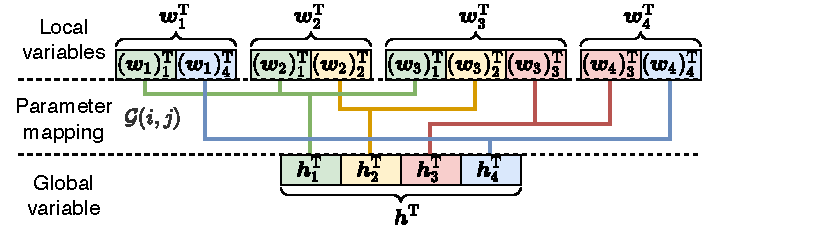
\includegraphics[trim={0.2cm 0.25cm 1.9cm 0.0cm},clip,width=\columnwidth]{images/parameter_mapping2.pdf}\label{fig:problem_splitting:parameter_mapping}}
    \vspace*{-0.1cm}
    \caption{(a) Network topology with 4 nodes. Arrows indicate exchange of signal information. (b) Data transmission between nodes \(i\) and \(j\) for each frame \(m\). (c) Parameter mapping of the local variable components \(({\wf}_i)_j\) to the global variable components \(\hf_j\) via \(\mathcal{G}(i,j)\) for the network in (a).}
    \label{fig:sensor_network:WSN_mapping}
\end{figure}

% #############################################################################
% #############################################################################
\section{Proposed Algorithm}
\label{sec:proposed_method}

% % #############################################################################
% \subsection{Problem Splitting}
% \label{ssec:problem_splitting}
% In state-of-the-art algorithms \cite{heNoiseRobustFrequencyDomain2018,habetsOnlineQuasiNewtonAlgorithm2010}, the minimization problem \eqref{eq:frequency_domain:min_prob} is solved in its full form resulting in potentially high computational effort when the number of channels and length of impulse responses or number of DFT bins is large.
% Here however, we split the problem into \(N \in \mathbb{N}\) sub-problems and denote the index set of these \(N\) sub-problems as \(\Nset \triangleq \{1,\ldots,N\}\).
% Each sub-problem is defined by a subset of the full channel set \(\Cset_i \subseteq \Mset\) with \(i \in \Nset\).
% Following from that, we define the sets \(\Csetb_j = \left\{ i \vert j \in \Cset_i \right\}\) for \(i,j \in \Mset\) where for each channel \(j\) a set represents the sub-problems that particular channel is part of.
% This channel-to-sub-problem relation can also be represented as a \(M \times N\) matrix \(\mtxb{G}\) where the sets \(\Cset_i\) and \(\Csetb_j\) are the indices of non-zero elements of the rows and columns respectively (see \autoref{fig:problem_splitting:problem_splitting_matrix}).
% Further, \(M_i = \left| \Cset_i \right| \) and \(N_j = \left| \Csetb_j \right| \) with \(i,j \in \Mset\).

% \begin{figure}
%     \centering
%     \subfloat[][]{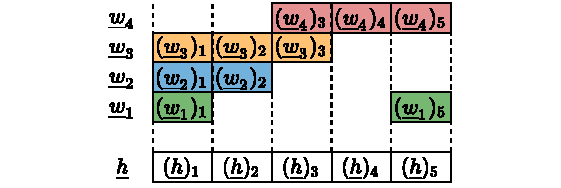
\includegraphics[trim={1.8cm 0 1.7cm 0},clip,scale=0.7]{images/parameter_mapping.pdf}}
%     \subfloat[][]{\includestandalone[trim={0.65cm 0 0 0},clip,scale=0.7]{tikz/connection_matrix}}
%     \subfloat[][]{\includestandalone[trim={0.6cm 0 0 0},clip,scale=0.6]{tikz/problem_splitting_matrix}}
%     % \includestandalone[scale=1]{tikz/topology_general}
%     \vspace*{-0.3cm}
%     \caption{Problem splitting and parameter mapping for a general case with \(M=5\) channels and \(N=4\) sub-problems. (a) shows the mapping of the local estimate components \((\wf_i)_j\) to the global consensus components \((\hf)_j\) via \(\mathcal{G}(i,j)\), (b) \(\mtxb{G}\) with 1 (\(\blacksquare\)) and 0 (\(\square\)), (c) shows \(i,j\)-cross-relations used by sub-problems compared to full \(M\)-channel problem.}
%     \label{fig:problem_splitting:problem_splitting_matrix}
% \end{figure}



% #############################################################################
\subsection{General-Form Consensus ADMM}
\label{ssec:general_consensus_admm}
Recall that in addition to its own signal information, each node \(i \in \Mset\) has access to that of nodes \(j \in \Rset_i\).
This is used to solve a BSI sub-problem of the same form as in \eqref{eq:frequency_domain:min_prob}, which only involves the subset of channels.
We define the local variables \(\wf_i = \left[ \left\{ (\wf_i)_j^\T \right\}_{j \in \Rset_i} \right]^\T\), which are stacked vectors of locally estimated frequency responses (cf. \autoref{fig:problem_splitting:parameter_mapping}).
Further, the global variable \(\hf = \begin{bmatrix}
    \hf_1^\T & \ldots & \hf_M^\T
\end{bmatrix}^\T\) is the stacked vector of all \(M\) channel response consensus variables.
Lastly, we define the matrix \(\hat{\aRhof}_i\), which is the frequency-domain cross-relation matrix analogous to \(\hat{\Rf}\) as introduced in \autoref{ssec:cross_rel}, however only using the signals \(\x_j\) with \(j \in \Rset_i\).

We replace the cost function minimized in \eqref{eq:frequency_domain:min_prob} with the separable cost function 
\begin{equation}
    \tilde{J}(\wf) = \sum_{i \in \Mset} \tilde{J}_i(\wf_i)  = \sum_{i \in \Mset} \wf_i^\herm \hat{\aRhof}_i \wf_i
    \label{eq:problem_splitting:cost_function}
\end{equation}
with \(\wf \triangleq (\wf_1,\ldots,\wf_M)\) as the local stacked estimates.
Minimization problems with separable cost functions, as introduced here, can be solved by the well-established method of consensus ADMM \cite{boydDistributedOptimizationStatistical2011}
\begin{equation}
    \begin{aligned}
        \underset{\wf,\,\hf}{\operatorname{minimize}} \quad &\sum_{i \in \Mset} \tilde{J}_i(\wf_i)\\
        \text{subject to} \quad &(\wf_i)_j = \hf_{\mathcal{G}(i,j)}\quad i \in \Mset,\,j \in \Rset_i\\
        &\hf^\herm \hf = 1
    \end{aligned}\label{eq:general_consensus_admm:min_prob}
\end{equation}
where \(\mathcal{G}(i,j)\) denotes the mapping of \(L\) local variable components \((\wf_i)_j\), i.e., one of the frequency responses in the stacked vector, to the corresponding global variable components \(\hf_j\) (cf. \autoref{fig:problem_splitting:parameter_mapping}).
For the sake of brevity, the mapped global variables \((\tilde{\hf}_i)_j = \hf_{\mathcal{G}(i,j)}\) are introduced.
This defines \(\tilde{\hf}_i = \left[ \left\{ \hf_j^\T \right\}_{j \in \Rset_i} \right]^\T\).
The equality constraint between local variables \(\wf_i\) and global variable \(\hf\) enforces consensus, i.e., a common solution taking into account estimates of all nodes that share data of the same channel.
The augmented Lagrangian for this particular general-form consensus problem is
\begin{equation}
    \begin{aligned}
        \mathcal{L}_{\rho} &(\wf,\hf,\uuf) = \sum_{i \in \Mset} \left( \wf_i^\herm \hat{\aRhof}_i \wf_i + 2 \Re \left( \uuf_i^{\herm} \left(\wf_i - \tilde{\hf}_i\right) \right)\right. \vphantom{+ \rho \left\| \wf_i - \tilde{\hf}_i \right\|^2}\\
        \vphantom{\wf_i^\herm \hat{\aRhof}_i \wf_i + 2 \Re \left( \uuf_i^{\herm} \left(\wf_i - \tilde{\hf}_i\right) \right)} & \qquad \qquad \qquad \qquad \left. + \rho \left\| \wf_i - \tilde{\hf}_i \right\|^2 \right)
    \end{aligned}\label{eq:general_consensus_admm:lagrangian}
\end{equation}
where \(\uuf \triangleq (\uuf_1,\ldots,\uuf_M)\) are the stacked local dual variables (Lagrange multipliers) \(\uuf_i = \left[ \left\{ (\uuf_i)_j^{\T} \right\}_{j \in \Rset_i} \right]^\T\) with \((\uuf_i)_j\) denoting the dual variable for channel \(j\) at node \(i\).
These variables follow from the consensus equality constraint in \eqref{eq:general_consensus_admm:min_prob}.
% The local variables \(\wf\) and global variable \(\hf\) are as introduced
The ADMM with penalty parameter/step size \(\rho > 0\) then consists of the steps \cite{boydDistributedOptimizationStatistical2011}:
\begin{align}
    \wf_i^{k+1} &= \underset{\wf_i}{\operatorname{argmin}} \, \mathcal{L}_{\rho} (\wf,\hf^k,\uuf^k)\label{eq:general_consensus_admm:local}\\
    \hf^{k+1} &= \underset{\hf, \|\hf\| = 1}{\operatorname{argmin}}\, \mathcal{L}_{\rho} (\wf^{k+1},\hf,\uuf^k)\label{eq:general_consensus_admm:global}\\
    \uuf_i^{k+1} &= \uuf_i^{k} + \rho \left( \wf_i^{k+1} - \tilde{\hf}_i^{k+1} \right),\label{eq:general_consensus_admm:dual}
\end{align}
where \(k\) is the iteration index. Evidently, this is an iterative algorithmand we will therefore introduce the online/adaptive aspect of the proposed algorithm in the following.

\subsection{Online ADMM-BSI}
\label{ssec:online_admm}
We introduced the original problem in \eqref{eq:frequency_domain:null_space} with a time-dependent estimate \(\hat{\Rf(m)}\) of the matrix \(\Rf(m)\). It therefore follows that the data term in \eqref{eq:general_consensus_admm:lagrangian} can also be considered time-dependent, which from here on will be denoted with the additional superscript time index \(m\) as \(\wf_i^\herm \hat{\aRhof}_i^{m} \wf_i\).
A thorough review of ADMM with time-varying data terms can be found in \cite{wangOnlineAlternatingDirection2013,hosseiniOnlineDistributedADMM2014} where it is referred to as ``Online-ADMM".
We transform the iterative batch processing method \eqref{eq:general_consensus_admm:local}-\eqref{eq:general_consensus_admm:dual} into an adaptive one by computing only a (small) finite number of iterations with each time-frame-\(m\) specific data term.
Here specifically, we apply one iteration per time frame, which manifests itself as simply replacing the iteration index \(k\) with the time frame index \(m\).

The minimization problem for the local variable \(\wf_i\) \eqref{eq:general_consensus_admm:local} can be solved by various algorithms, in this case however we perform the adaptive update step as
\begin{equation}
    \wf_i^{m+1} = \wf_i^{m} - \mu \bm{{V}}_i^m \left( \hat{\aRhof}_i^m \wf_i^m + \uuf_i^m + \rho\left(\wf_i^m - \tilde{\hf}_i^{m}\right)\right),\label{eq:online_admm:local_update}
\end{equation}
where \(\mu\), (\(0  < \mu\leq 1\)), is a step size and \(\bm{{V}}_i^m = \left(\hat{\aRhof}_i^m + \rho \I \right)^{-1}\) is the regularized inverse Hessian of the problem.
The implicit overlap-save matrices in \(\bm{{V}}_i^m\) make this a constrained update step which is costly to compute, so in order to reduce computational complexity, we introduce the approximation
\begin{equation}
    \hat{\bm{{V}}}_i^m = \operatorname{diag} \left\{ \operatorname{diag} \left\{ \hat{\aRhof}_i^m \right\} + \rho \mtxb{1} \right\}^{-1},
\end{equation}
which is straightforward to compute.
It may be readily verified (cf. \cite{boydDistributedOptimizationStatistical2011}) that the solution to \eqref{eq:general_consensus_admm:global} is given by an update step which computes
\begin{equation}
    \hf_i^{m+1} = \frac{\bar{\hf}_i^{m+1}}{\sqrt{\sum_{j \in \Tset_i} \|\bar{\hf}_i^{m+1}\|^2}}\label{eq:online_admm:consensus_update}
\end{equation}
for each node \(i \in \Mset\) with the local unnormalized consensus
\begin{equation}
    \bar{\hf}_i^{m+1} = \bar{\wf}_i^{m+1} + \frac{1}{\rho} \bar{\uuf}_i^{m}.
\end{equation}
Here, \(\bar{\wf}_i = \frac{1}{N_i} \sum_{j \in \Tset_i} (\wf_j)_i\) and \(\bar{\uuf}_i = \frac{1}{N_i} \sum_{j \in \Tset_i} (\uuf_j)_i\), with \(N_i = | \Tset_i |\), are neigborhood averages of the channel response estimate and the dual variable of channel \(i\) respectively, computed at node \(i\). The values of all \(\|\bar{\hf}_i^{m+1}\|^2\), \(i \in \Mset\) are transmitted and relayed through the network until all nodes can compute the denominator in \eqref{eq:online_admm:consensus_update}.
Finally, the update of the dual variables is given by
\begin{equation}
    \uuf_i^{m+1} = \uuf_i^{m} + \rho \left( \wf_i^{m+1} - \tilde{\hf}_i^{m+1} \right).\label{eq:online_admm:dual_update}
\end{equation}
The computations of local, consensus, and dual variables in \eqref{eq:online_admm:local_update}, \eqref{eq:online_admm:consensus_update} and \eqref{eq:online_admm:dual_update} respectively, require data transmitted by other nodes (cf. \autoref{fig:sensor_network:WSN_detail}). For this paper, we assume that all transmissions are done instantaneously whenever variables are required by neighboring nodes and are error-free.

% \autoref{alg:dbsi} presents the full algorithm including inter-node transmissions.

% \begin{algorithm}
%     \caption{Distributed BSI with ADMM}\label{alg:dbsi}
%     \begin{algorithmic}
%         \For {\(m=0,1,2,...\)}
%             \For{\(i \in \Mset\)}
%                 \State Acquire signal vector \(x_i^{(m)}\)
%                 \ForAll{\(j \in \Tset_i\)}
%                     \State Send \(x_i^{(t)},\bar{h}_i^{(t)},\bar{y}_i^{(t)}\) to node \(j\)
%                 \EndFor
%                 \ForAll{\(k \in \mathcal{R}_i\)}
%                     \State Receive \(x_{k}^{(t)},\bar{h}_{k}^{(t)},\bar{y}_{k}^{(t)}\) from node \(k\)
%                 \EndFor
%                 \State Update \(\phi_i^{(t+1)} \leftarrow \phi_i^{(t)}\) using \eqref{eq:admm_local}
%                 \State Update \(\gamma_i^{(t+1)} \leftarrow \gamma_i^{(t)}\) using \eqref{eq:admm_consensus}
%                 \State Update \(\lambda_i^{(t+1)} \leftarrow \lambda_i^{(t)}\) using \eqref{eq:admm_dual}
%                 \ForAll{\(k \in \mathcal{R}_i\)}
%                     \State Send \(\hat{h}_{ki}^{(t)},y_{ki}^{(t)}\) to node \(k\)
%                 \EndFor
%                 \ForAll{\(j \in \Tset_i\)}
%                     \State Receive \(\hat{h}_{ij}^{(t)},y_{ij}^{(t)}\) to node \(j\)
%                 \EndFor
%             \EndFor
%         \EndFor
%     \end{algorithmic}
% \end{algorithm}

% For the update step of the consensus variable \(\hf\), it may be readily verified (cf. \cite{boydDistributedOptimizationStatistical2011}) that the solution to \eqref{eq:general_consensus_admm:global} is given by
% \begin{equation}
%     \hf^{m+1} = \frac{\bar{\wf}^{m+1} + \frac{1}{\rho} \bar{\uuf}^{m} }{\left\| \bar{\wf}^{m+1} + \frac{1}{\rho} \bar{\uuf}^{m} \right\|}.\label{eq:online_admm:consensus_update}
% \end{equation}
% where the \(M L \times 1\) vectors \(\bar{\wf}^{m+1}, \bar{\uuf}^{m+1}\) are computed as the mapped averages
% \begin{equation}
%     (\bar{\wf}^{m+1})_g = \frac{1}{N_g} \sum_{\mathcal{G}(i,j)=g} (\wf_i^{m+1})_j,\quad g,i \in \Mset, \, j \in \Tset_g
% \end{equation}
% and
% \begin{equation}
%     (\bar{\uuf}^{m})_g = \frac{1}{N_g} \sum_{\mathcal{G}(i,j)=g} (\uuf_i^{m})_j,\quad g,i \in \Mset, \, j \in \Tset_g
% \end{equation}
% with \(N_g = | \Tset_g |\) being the cardinality of the set.
% This results in a computationally inexpensive update step forcing the norm of the consensus to have unit value.

% #############################################################################
% #############################################################################
\section{Numerical Evaluation}
\label{sec:perf_eval}

\begin{figure}[t]
    \centering
    \hspace*{-0.2cm}\subfloat[][]{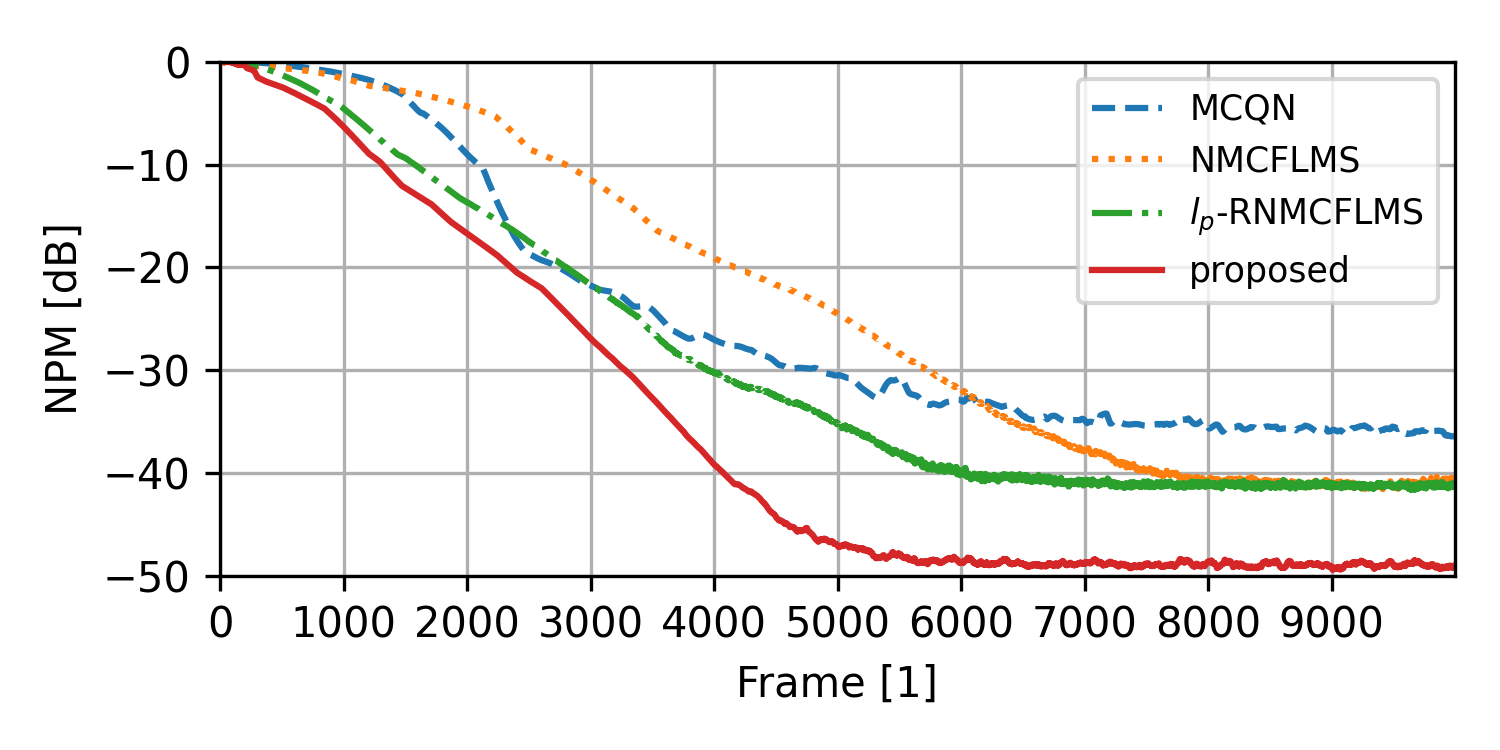
\includegraphics[trim={0.3cm 0.35cm 0.3cm 0.3cm},clip,height=4cm]{python/simulation_1/plots/NPM_over_time_SNR20.png}\label{fig:perf_eval:NPM_over_time_SNR20}}\\
    \vspace*{-0.3cm}
    \hspace*{-0.2cm}\subfloat[][]{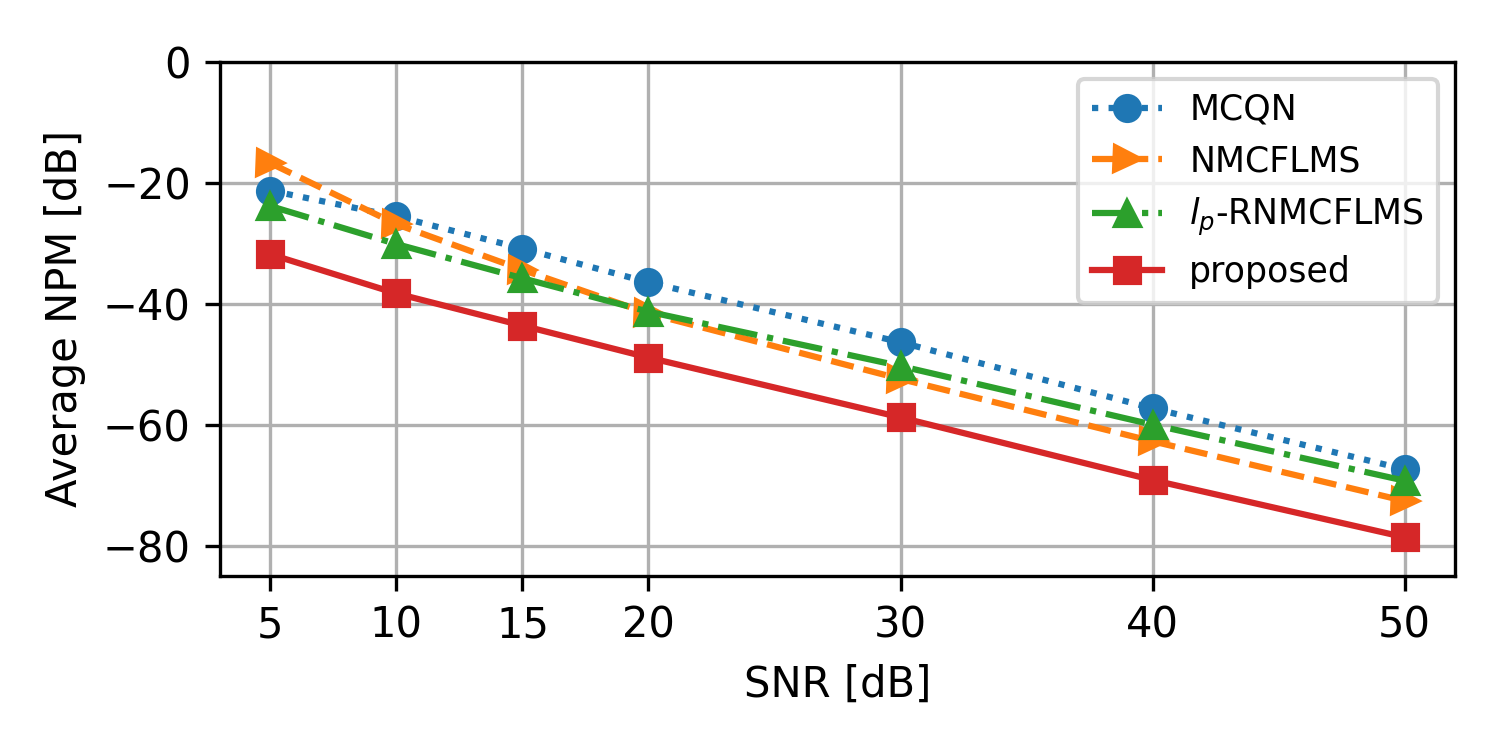
\includegraphics[trim={0.3cm 0.35cm 0.3cm 0.3cm},clip,height=4cm]{python/simulation_1/plots/NPM_over_SNR_L64_M5.png}\label{fig:perf_eval:NPM_over_SNR_L64_M5}}
    \vspace*{-0.2cm}
    \caption{(a) NPM at \(\text{SNR}=20\,\text{dB}\) over frame index \(m\) and (b) steady-state NPMs over different SNRs.}
    \label{fig:perf_eval:NPM_over_time_exp1}
\end{figure}

The performance of the proposed algorithm is assessed via numerical simulations.
As an error measure, we use the normalized projection misalignment (NPM) \cite{huangClassFrequencydomainAdaptive2003}
% \begin{equation}
%     \text{NPM}(m) = 20\,\log_{10} \left(\frac{\left\| \h(m) - \frac{\h^\T (m) \h_{\text{t}}}{\h_{\text{t}}^\T \h_{\text{t}}}\h(m) \right\|_2}{\left\|\h(m)\right\|_2} \right)
% \end{equation}
\begin{equation}
    \text{NPM}(m) = 20\,\log_{10} \left(\left\| \h(m) - \frac{\h^\T (m) \h_{\text{t}}}{\h_{\text{t}}^\T \h_{\text{t}}}\h(m) \right\| / \left\|\h(m)\right\| \right),
\end{equation}
where \(\h\) is the stacked vector of impulse response estimates (cf. \autoref{ssec:cross_rel}), which are the inversely Fourier-transformed estimated frequency responses \(\hf_i\) stacked in \(\hf\) and \(\h_{\text{t}}\) is the ground truth. The signal-to-noise ratio (SNR) for the simulations is defined as 
\begin{equation}
    \text{SNR} = 10 \log_{10} \left(\frac{\sigma_s^2 \| \h_t \|}{M \sigma_v^2} \right),
\end{equation}
where \(\sigma_s^2\) and \(\sigma_v^2\) are the variance of signal and noise respectively which for this paper both are modelled by (channel-independent) white Gaussian noise (WGN).

For this paper, the first simulation evaluates the performance using randomly generated impulse responses of length \(L=64\) under different signal-to-noise ratios (SNR) on a 5-node network (5-channel system, \(M=5\)) with a ring topology where each node transmits its signal information to one neighbor.
The impulse responses are drawn from a zero-mean Gaussian distribution with unit variance, and the signal is \(8\!\times\!10^{5}\) samples of WGN to ensure convergence of all algorithms.
The step sizes are hand-tuned, so that the steady state is reached at similar frame counts (or later than the proposed algorithm): \(\mu_{\text{MCQN}}=0.01,\,\mu_{\text{NMCFLMS}}=0.3,\,\mu_{l_p-\text{NMCFLMS}}=0.4,\,\mu_{\text{ADMM}}=0.6,\,\rho=1,\,\eta=0.98 \).
\autoref{fig:perf_eval:NPM_over_time_SNR20} shows the median NPM (30 Monte-Carlo runs) over frame index \(m\).
\autoref{fig:perf_eval:NPM_over_SNR_L64_M5} shows the median (30 Monte-Carlo runs) where the averaged NPM of \(100\) frames after convergence is plotted.
It can be observed that the proposed algorithm yields a lower steady-state NPM than the compared NMCFLMS, RNMCFLMS, and \(l_p\)-RNMCFLMS algorithms.
The choice to present the median is based on the fact that randomly generated impulse responses may have (near) common zeros which diminish the identifiability of these systems \cite{naylorNearCommonZerosBlind2008}, here considered outliers.


\begin{figure}[t]
    \centering
    % \hspace*{-0.2cm}\subfloat[][\(M\!=\!4\)]{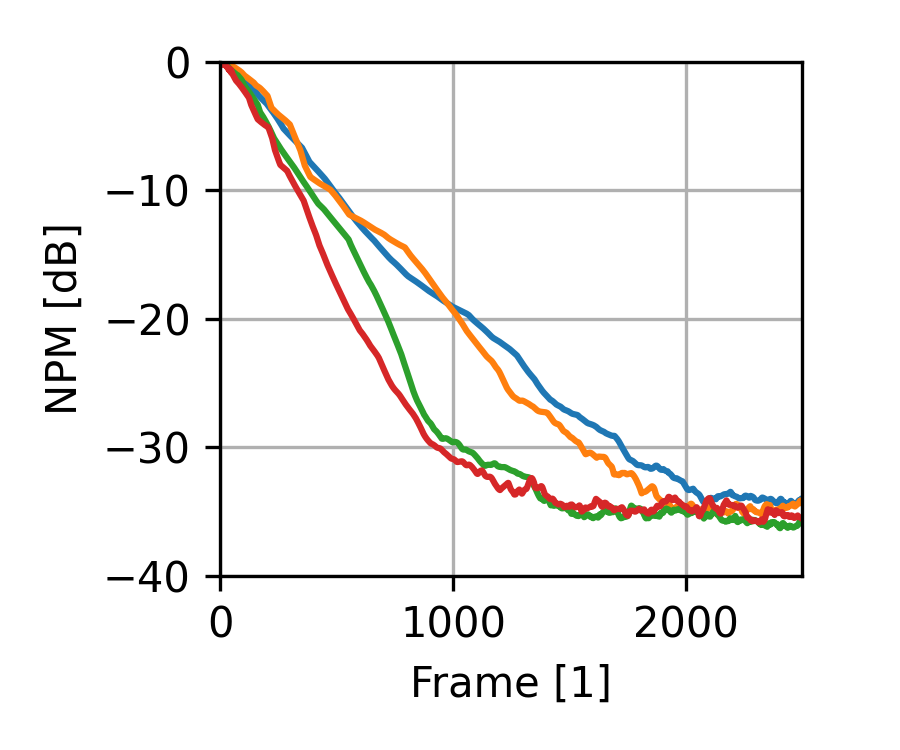
\includegraphics[trim={0.3cm 0.35cm 0.3cm 0.3cm},clip,height=3.7cm]{python/plots/NPM_over_time_M4.png}\label{fig:perf_eval:NPM_over_time_M4}}
    \hspace*{-0.1cm}\subfloat[][]{\begin{overpic}[trim={0.3cm 0.35cm 0.8cm 0.3cm},clip,height=4cm]{python/simulation_2/plots/NPM_over_time_M4.png}
        \put(60,53){\includestandalone[trim={0.0cm 0.0cm 0.0cm 0},clip,scale=0.6]{tikz/topology_inset_simulation}}
    \end{overpic}\label{fig:perf_eval:NPM_over_time_M4}}
    \hspace*{0.3cm}\subfloat[][]{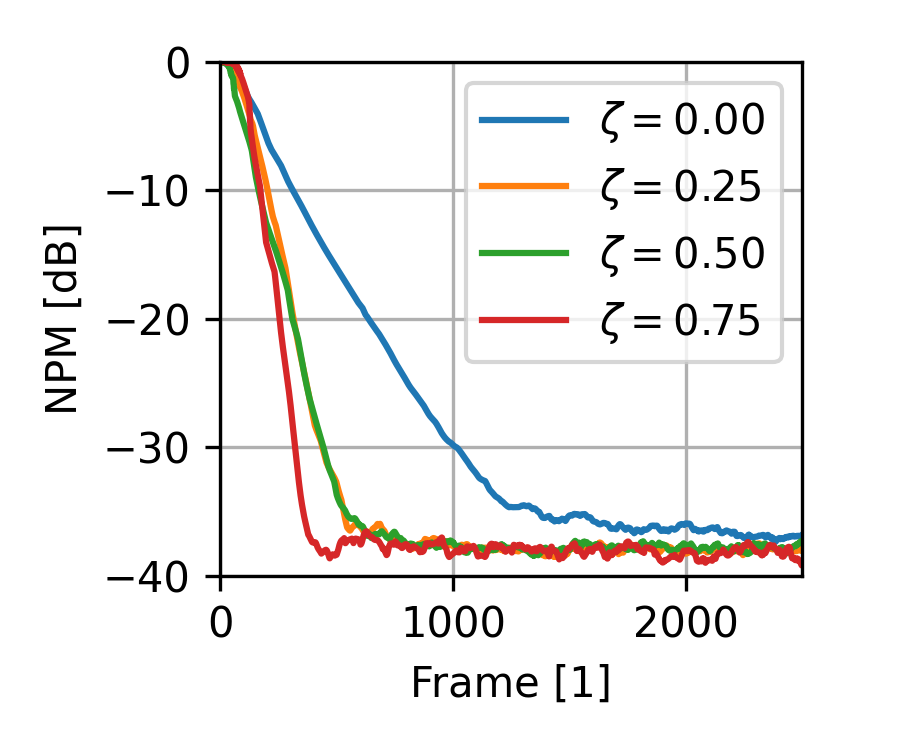
\includegraphics[trim={0.3cm 0.35cm 0.8cm 0.3cm},clip,height=4cm]{python/simulation_2/plots/NPM_over_time_M8.png}\label{fig:perf_eval:NPM_over_time_M8}}
    \vspace*{-0.2cm}
    \caption[Convergence behaviour with \(L\!=\!16\) for different values of \(\zeta\)]{Convergence behaviour with \(L\!=\!16\) for different values of \(\zeta\) for \(\text{SNR}=20\,\text{dB}\). NPM for systems of (a) 4 nodes/channels and (b) 8 nodes/channels. The inset of (a) shows the base ring topology (black arrows) and all other possible connections (dashed black arrows).}
    \label{fig:perf_eval:NPM_over_time_exp2}
\end{figure}

The second simulation is a small-scale assessment of the influence of the number of connections within the WSN.
Two base scenarios, \(M=4\) and \(M=8\) are evaluated using short (\(L=16\)) random impulse responses and with semi-random topologies.
Each topology is generated by forming a ring topology as marked with solid arrows on the inset of \autoref{fig:perf_eval:NPM_over_time_M4} and additionally randomly selecting a defined number of connections from all remaining possible connections, marked with dashed arrows.
The parameter \(\zeta\) is defined as the ratio of randomly selected connections to possible connections (excluding the ring topology).
Topologies satisfying this definition for \(\zeta \in \{0.0,\,0.25,\,0.5,\,0.75\}\) were generated.
\autoref{fig:perf_eval:NPM_over_time_M4} and \autoref{fig:perf_eval:NPM_over_time_M8} show the median NPM (30 Monte-Carlo runs) for \(M=4\) and \(M=8\) respectively. The plots suggest a proportional relation between convergence speed, channel number \(M\) and \(\zeta\). Moreover, the steady-state error appears to be independent of \(\zeta\).

% #############################################################################
% #############################################################################
\section{Conclusions}
\label{sec:conclusion}
In this paper, a distributed adaptive algorithm for blind system identification using ADMM in the context of sensor networks was developed.
The BSI problem is distributed amongst the nodes by exploiting the separability of the cross-relation problem formulation which leads to node-wise sub-problems using signal information of a node's neighborhood.
The nodes solve the subproblem and transmit estimates to their respective neighbors which are combined into consensus estimates.
Preliminary results using white Gaussian noise and randomly generated impulse responses have demonstrated improved steady-state error measures compared to state-of-the-art algorithms.
Further, they suggest that steady-state performance is not affected by the separation of the full BSI problem into node-wise sub-problems while convergence speed is.

% References should be produced using the bibtex program from suitable
% BiBTeX files (here: strings, refs, manuals). The IEEEbib.bst bibliography
% style file from IEEE produces an unsorted bibliography list.
% -------------------------------------------------------------------------
\bibliographystyle{IEEEbib}
\bibliography{refs}

\end{document}